\chapter{Series de potencias. Productos infinitos}
\label{cap:ejemplos}

% Introducción

\section{Ejemplos de series de potencias}
\label{sec:ejemplos}

En esta sección vamos a estudiar el comportamiento de algunas series de potencias en el borde de su disco de convergencia. Para ello primero vamos a recordar algunos conceptos que nos van a ser de utilidad. Sea $f(z)$ una serie de potencias con coeficientes $\{a_n\}_{n=1}^{\infty} \subset \complex$ centrada en $z_0$ dada por
\begin{equation*}
    f(z) =  \sum_{n=0}^\infty a_n (z-z_0)^n,
\end{equation*}
donde $z \in \complex$. \\

\begin{definition}
    Se llama radio de convergencia de una serie de potencias a
    \begin{equation*}
        R = \sup \left\{ \abs{z - z_0} : \sum _{n=0}^{\infty} a_n (z - z_0)^n \text{ converge } \right\} \in [0, \infty].
    \end{equation*}
\end{definition}
\medskip

Cuando el radio de convergencia cumple que $0 < R < \infty$, $R$ es el único número real tal que la serie converge si $\abs{z - z_0} < R$, y diverge si $\abs{z - z_0} > R$. Por ello, decimos que $D(z_0,r)$ es el disco de convergencia de la serie. \\

En la frontera del disco de convergencia, esto es, cuando $\abs{z - z_0} = r$, el comportamiento de la serie de potencias puede ser complicado, es decir, puede converger para unos valores de $z$ y divergir para otros. \\

Todas las series que vamos a presentar tienen radio de convergencia $1$ y están centradas en el origen. Sin embargo, cada una de ellas muestra una situación diferente relacionada con su comportamiento en la frontera del disco unidad. \\

%%%%%%%%%%%%%%%%%%%%%%%%%%%%%%%%%%%%%%%%%%%%%%%%%%%%%%%%%%%%%%%%%%%%%%%%%%%%%%%%
%EJEMPLO 1
%%%%%%%%%%%%%%%%%%%%%%%%%%%%%%%%%%%%%%%%%%%%%%%%%%%%%%%%%%%%%%%%%%%%%%%%%%%%%%%%

En primer lugar tenemos la serie geométrica, una serie con radio de convergencia $1$, no acotada y que no converge en ningún punto de la frontera de su disco de convergencia. Sin embargo, la serie puede extenderse a una función globalmente analítica en $\complex \setminus \{1\}$ mediante una cantidad finita de prolongaciones analíticas. \\


\begin{example}
    Mostrar que
    \begin{equation*}
        \sum_{n=0}^{\infty} z^n, \, \abs{z} < 1
    \end{equation*}
    diverge en todo punto tal que $\abs{z} = 1$.
\end{example}

\begin{proof}
Es fácil ver que $1 - z^{n+1} = (1 - z) (1+ z + z^2 + \cdots + z^n)$. Por lo tanto, si $z \neq 1$, se tiene que
\begin{equation}
    1 + z + \cdots + z^n = \frac{1 - z^{n+1}}{1-z}.
\end{equation}

Por un lado, si $\abs{z} < 1$ entonces $\lim_{n \to \infty} z^n = 0$ y la serie converge a
\begin{equation*}
    \sum_{n=0}^{\infty} z^n = \frac{1}{1 - z}.
\end{equation*}

Ahora bien, si $\abs{z} > 1$ entonces $\lim_{n \to} z^n = \infty$ y la serie diverge. Pero, ¿qué pasa cuando $\abs{z} = 1$? La serie de potencias $\sum_{n=0}^{\infty} z^n$ diverge en todos los puntos del radio de convergencia pues $\abs{z^n}$ no tiende a 0 cuando $n \to \infty$. \\

Sin embargo, $\sum_{n=0}^{\infty} z^n$ puede ser extendida a la función globalmente analítica $\frac{1}{1-z}$ en $\complex \setminus \{1\}$ gracias a una cantidad finita de prolongaciones analíticas. \\

Tomemos $a$ un punto cualquiera de $\complex \setminus \{1\}$ y conectémoslo al origen $0$ mediante la curva de Jordan $\gamma \subset \complex \setminus \{1\}$. Fijemos un punto $z_1$ en $\gamma$ que cumpla $\abs{z} < 1$. $\sum_{n=0}^{\infty} z^n$ puede ser extendida analíticamente en $z_1$ de la siguiente forma:
\begin{equation*}
    \begin{split}
        \frac{1}{1-z} & = \frac{1}{1 - z_1 - (z - z_1)} = \frac{1}{1 - z_1} \frac{1}{1 - \frac{z - z_1}{1 - z_1}} = \frac{1}{1 - z_1} \sum_{n=0}^{\infty} \left(\frac{z - z_1}{1 - z_1} \right)^n = \\
                      & = \sum_{n=0}^{\infty}  \frac{1}{(1 - z_1)^{n+1}} (z - z_1)^n, \abs{z - z_1} < \abs{1 - z_1}.
    \end{split}
\end{equation*}

De nuevo, tomemos $z_2$ en $\gamma$ tal que $\abs{z_2 - z_1} < \abs{1 - z_1}$ y $\abs{z_2} \geq 1$. Podemos extender la serie de potencias a $z_2$ de la misma forma:
\begin{equation*}
    \frac{1}{1-z} = \sum_{n=0}^{\infty} \frac{1}{(1 - z_2)^{n+1}} (z - z_2)^n , \abs{z - z_2} < \abs{1 - z_2}.
\end{equation*}

Después de un número finito de iteraciones, dado que la curva es un conjunto compacto, alcanzaremos el punto $a$ y tendremos
\begin{equation*}
    \frac{1}{1-z} = \sum_{n=0}^{\infty} \frac{1}{(1 - a)^{n+1}} (z - a)^n , \abs{z - a} < \abs{1 - a}.
\end{equation*}

Así, decimos que hemos obtenido la prolongación analítica de $\sum_{n=0}^{\infty} z^n$ que pasa por la curva $\gamma$. \\

\begin{figure}[!htbp]
    \centering
    \begin{tikzpicture}[scale=0.8, use Hobby shortcut]
        \draw (4, 1) circle (3.1622776601683795cm);
        \draw (0, 0) circle (1cm);
        \draw (0.8377223398316204 ,1) circle (1.01308145723319cm);
        \draw (0.19918404494511877, 0.5989105159617241) circle (1cm);

        \filldraw (0, 0) circle (1pt) node[below, font=\scriptsize]{$z_0 = 0$};
        \filldraw (0.19918404494511877, 0.5989105159617241) circle (1pt) node[below right=-0.1, font=\scriptsize]{$z_1$};
        \filldraw (0.8377223398316204, 1) circle (1pt) node[below right=-0.15, font=\scriptsize]{$z_2$};
        \filldraw (4, 1) circle (1pt) node[below, font=\scriptsize]{$z_m = a$};
        \filldraw (1, 0) circle (1pt) node[below, font=\scriptsize]{$1$};

        \draw (0, 0) .. (0.19918404494511877, 0.5989105159617241) .. (0.8377223398316204, 1) .. (4, 1);
        \node[above, font=\footnotesize] at (2.5, 1.2) {$\gamma$};
    \end{tikzpicture}
    \caption{Prolongaciones analíticas.}
    \label{fig:prolongacion}
\end{figure}

Podemos hacer uso de la aplicación que se ha desarrollado como complemento para visualizar con mayor claridad el comportamiento de esta función en el disco unidad. La figura \ref{fig:ejemplo1} muestra la función globalmente analítica $\frac{1}{1-z}$ en $\partial \disk \setminus \{1\}$. \\

\begin{figure}[!htbp]
    \centering
    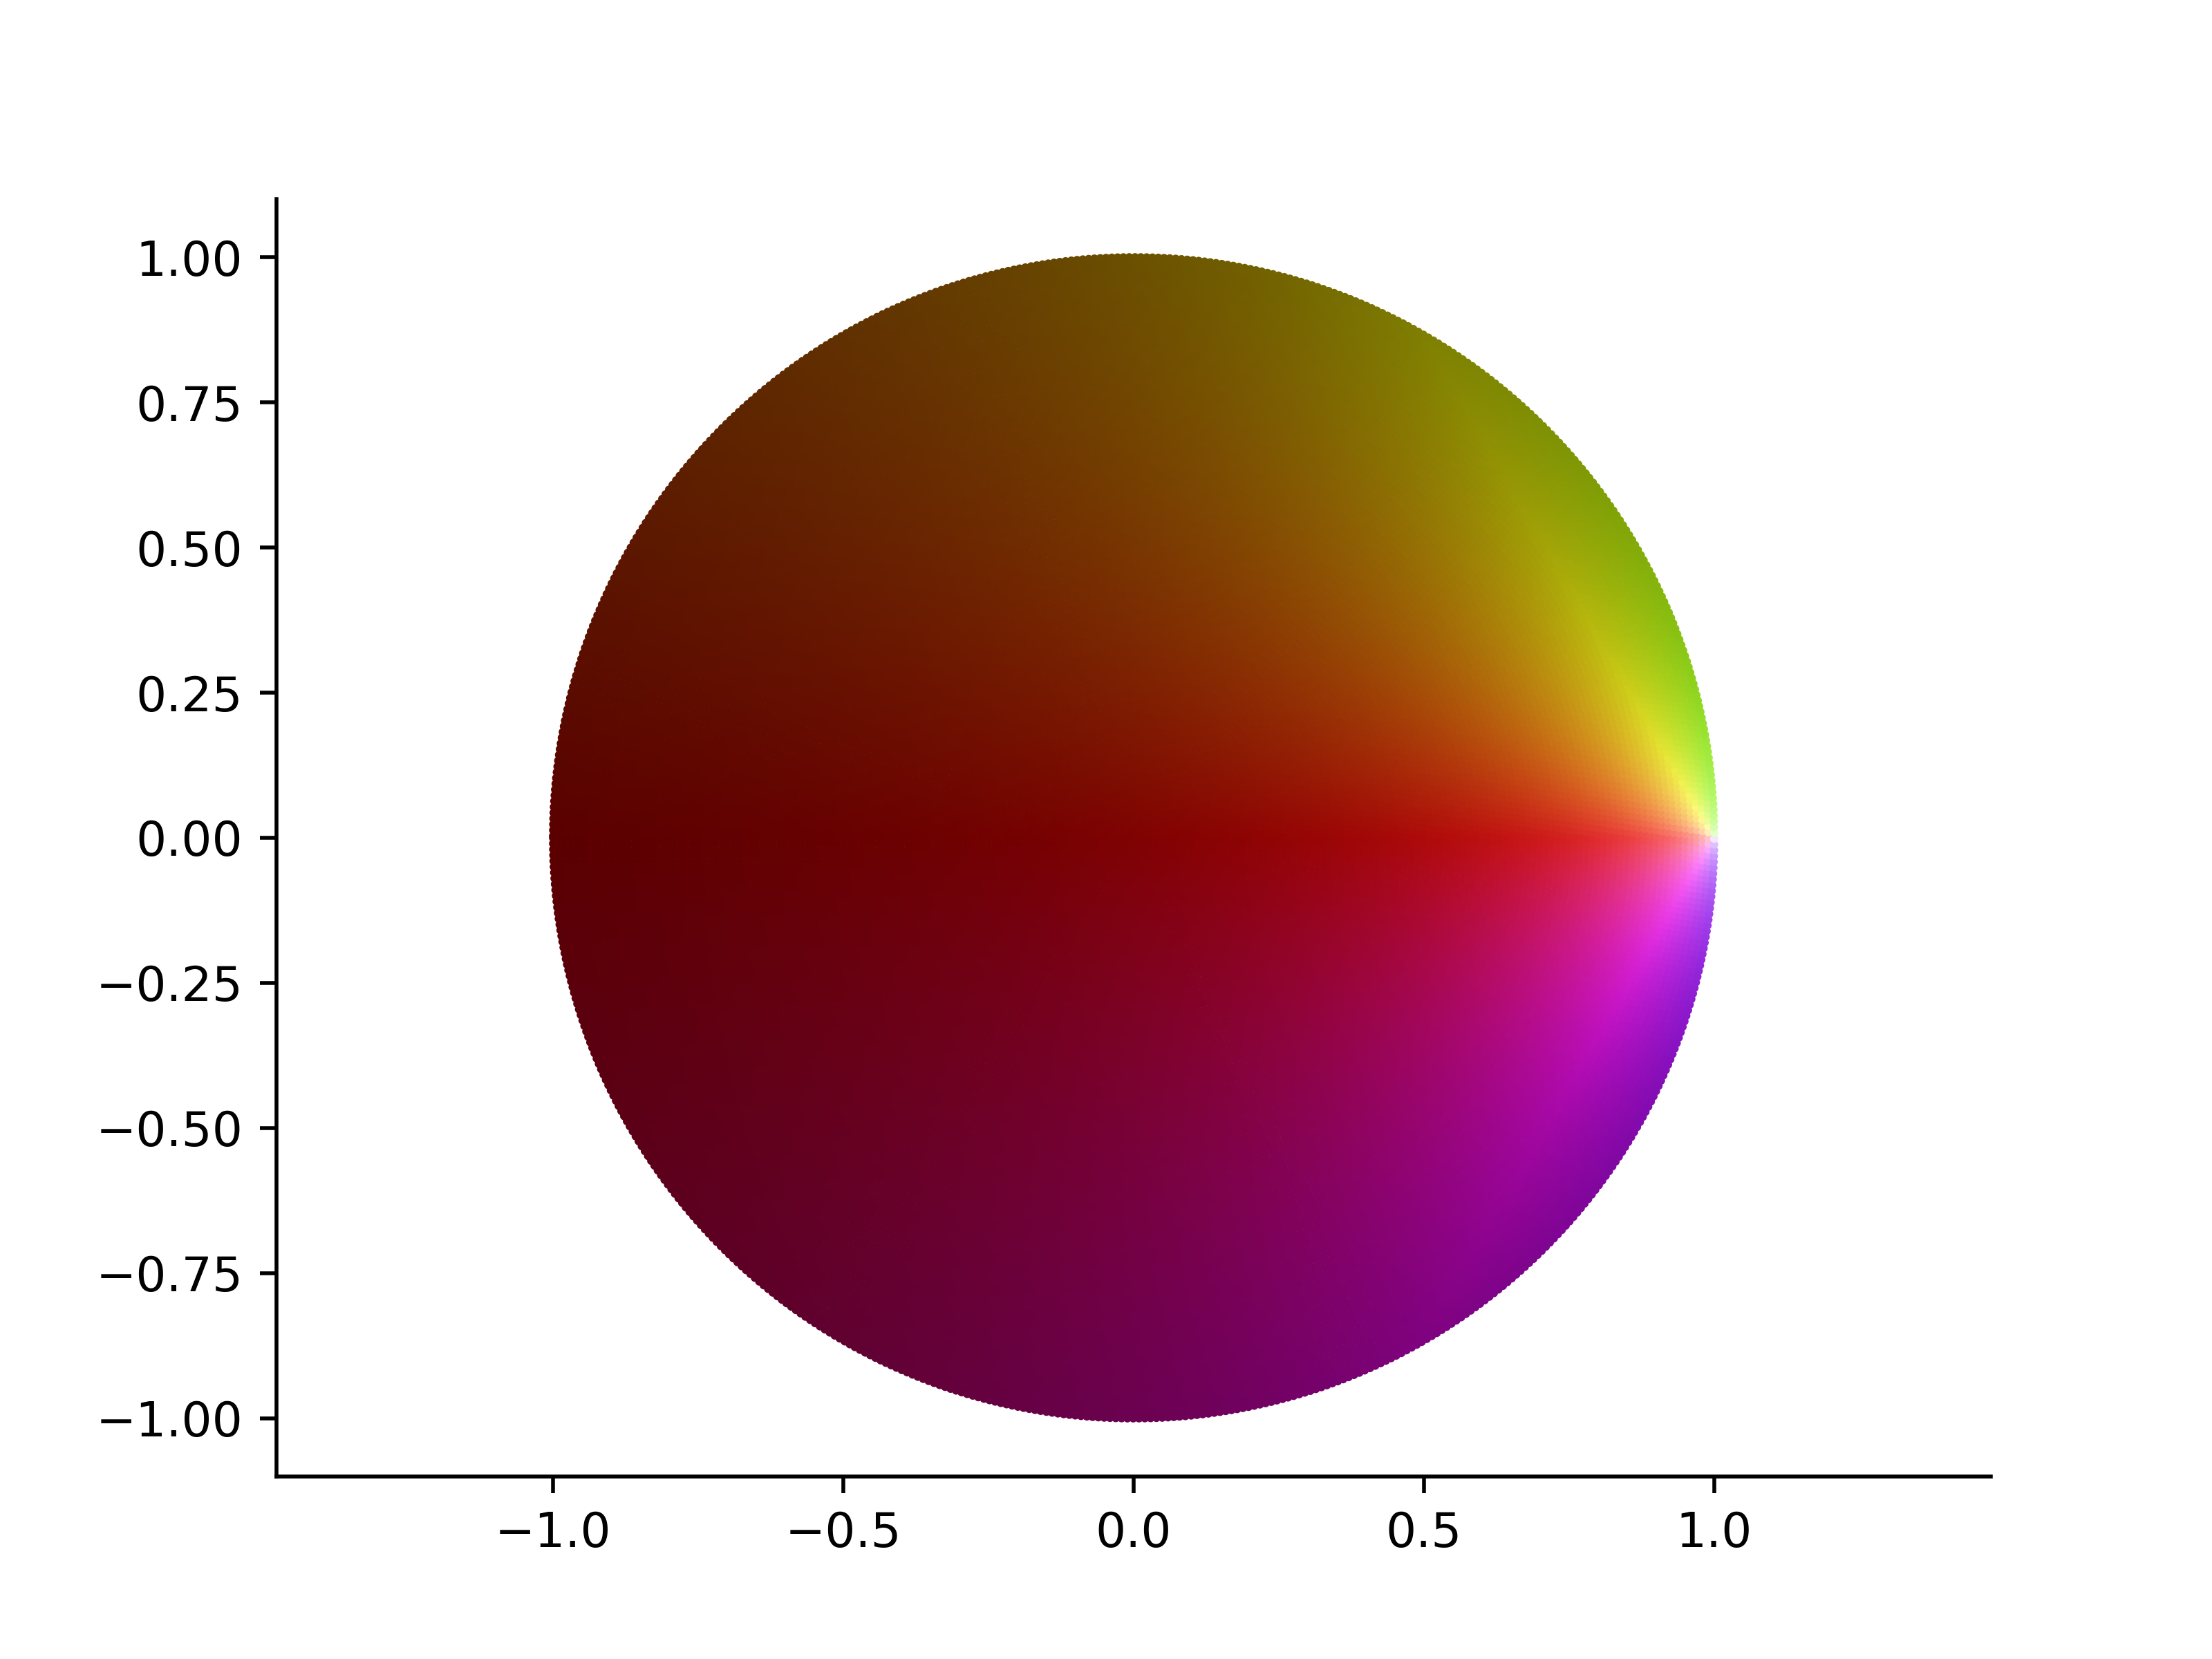
\includegraphics[width=0.7\textwidth]{../Aplicacion/1:(1-z).png}
    \caption{Representación de la función $\frac{1}{1-z}$ en el disco unidad.}
    \label{fig:ejemplo1}
\end{figure}
\end{proof}

%%%%%%%%%%%%%%%%%%%%%%%%%%%%%%%%%%%%%%%%%%%%%%%%%%%%%%%%%%%%%%%%%%%%%%%%%%%%%%%%
%EJEMPLO 2
%%%%%%%%%%%%%%%%%%%%%%%%%%%%%%%%%%%%%%%%%%%%%%%%%%%%%%%%%%%%%%%%%%%%%%%%%%%%%%%%

A continuación, presentamos otra serie con radio de convergencia $1$, que converge en todos los puntos del borde salvo en $z = 1$. Además, podemos expresar la suma de esta serie en términos de la serie anterior si $z \not = 1$. \\

\begin{example}
    Mostrar que
    \begin{equation*}
        g(z) = \sum_{n=1}^{\infty} \frac{z^n}{n}, \, \abs{z} < 1
    \end{equation*}
    diverge en $z = 1$  y converge en el resto de punto tales que $\abs{z} = 1$;

\end{example}

\begin{proof}
    En primer lugar, cabe destacar que la serie armónica $\sum_{n=1}^{\infty} \frac{1}{n}$ diverge, por lo que la serie de nuestro ejemplo diverge para $z = 1$. Para demostrar que la serie converge en el resto de punto tales que $\abs{z} = 1$ vamos a aplicar el criterio de Dirichlet, que recordamos a continuación. \\

    Sean $\{a_n\} \subset \real$ y $\{b_n\} \subset \complex$ sucesiones tales que:
    \begin{enumerate}
        \item $\{a_n\}$ es monótona con límite $0$
        \item Las sumas parciales de la serie $\sum_{n=1}^{\infty} b_n$ están acotadas
    \end{enumerate}
    entonces $\sum_{n=1}^{N} a_nb_n$ converge. \\

    En nuestro caso vamos a tomar $a_n = \frac{1}{n}$ y $b_n = z^n$. La primera condición se cumple, veamos la que resta:
    \begin{equation*}
        \abs{\sum_{n=1}^{N} z^n} = \abs{\frac{z - z^{N+1}}{1 - z}} \leq \frac{2}{\abs{1 - z}},
    \end{equation*}
    si $z \neq 1$, para todo $N \in \naturals$. \\

    Esto muestra que la condición se satisface para todo $z \not = 1$ en el disco unidad. Por lo tanto, la serie converge para todo $z$ tal que $\abs{z} \leq 1, z \not = 1$ y diverge para $\abs{z} > 1$. \\

    Vamos a ver que la suma de la serie es $\log{\frac{1}{1 - z}}$ cuando $z \not = 1$. En efecto, derivando tenemos que
    \begin{equation*}
        g'(z) = \sum_{n=1}^{\infty} z^{n-1} \Rightarrow z g'(z) = \sum_{n=1}^{\infty} z^n = \frac{z}{1 - z}.
    \end{equation*}
    Si integramos ahora la expresión de la derecha tenemos que la suma es $\log{\frac{1}{1 - z}}$ puesto que $g(0) = 0$. \\

    De nuevo, haciendo uso de la aplicación, hemos generado la figura  \ref{fig:ejemplo2} que muestra la función $\log{\frac{1}{1 - z}}$ en $\partial \disk$. \\

\begin{figure}[!htbp]
    \centering
    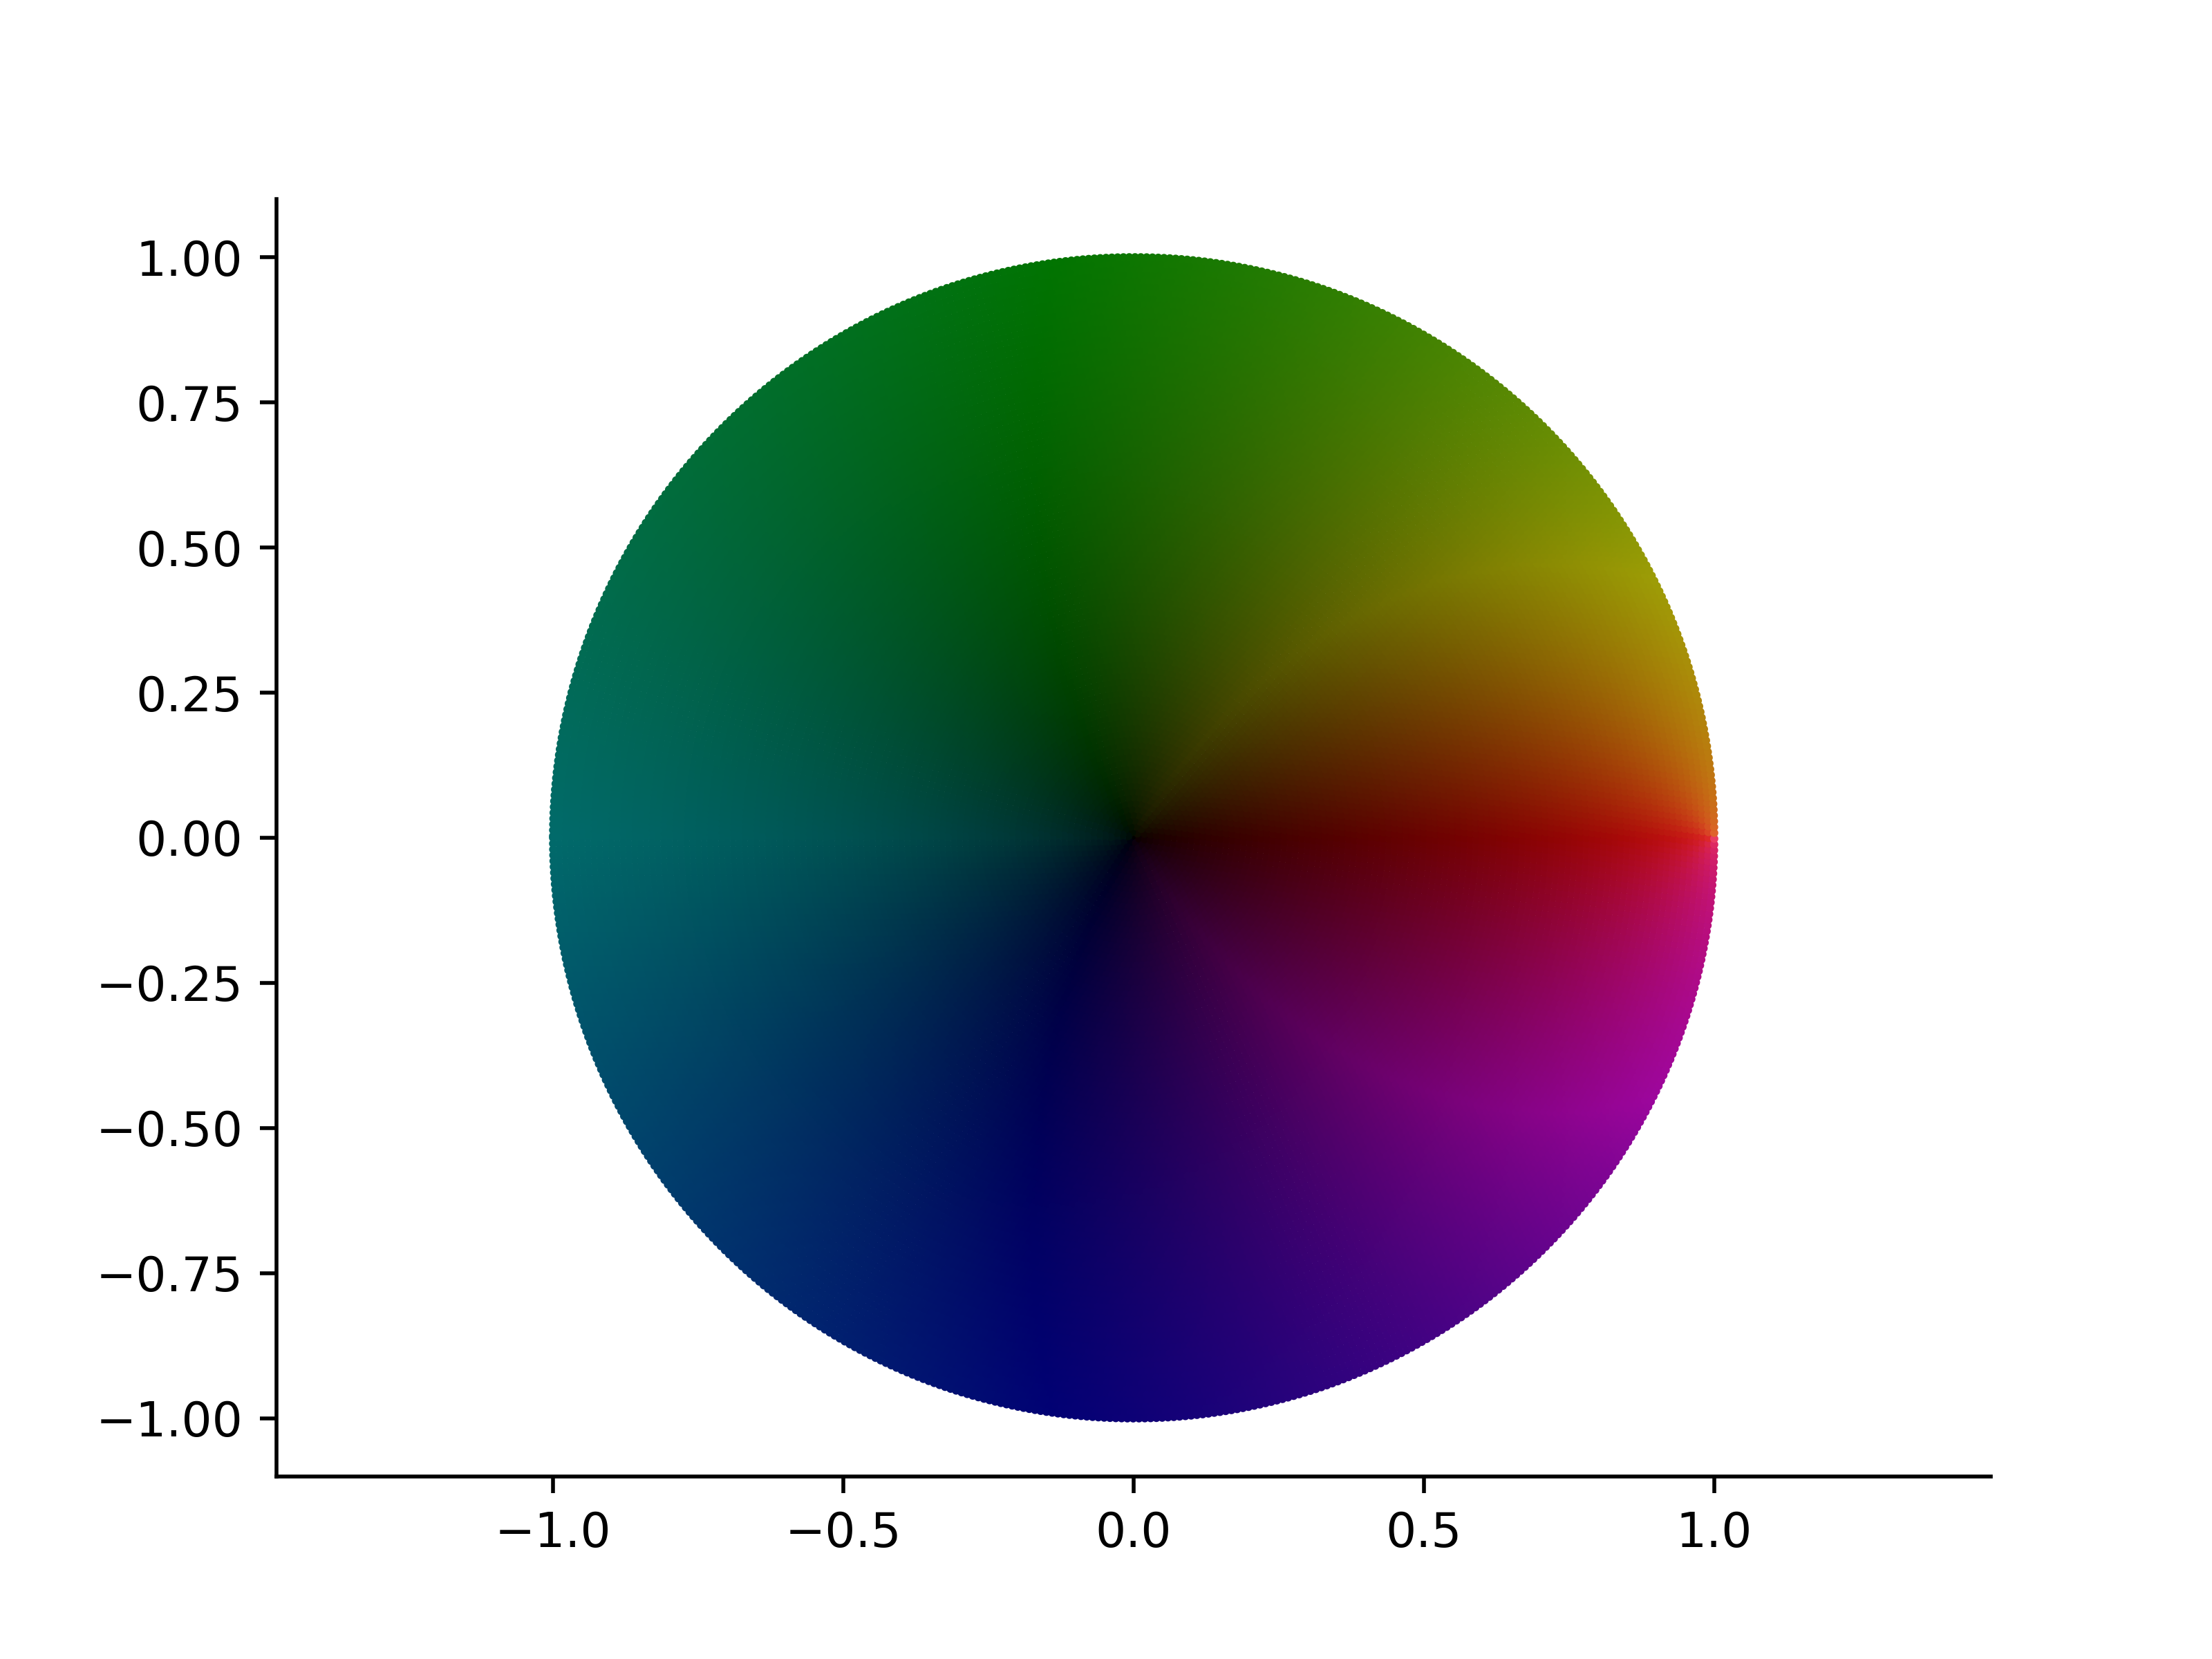
\includegraphics[width=0.7\textwidth]{../Aplicacion/log(1:(1-z)).png}
    \caption{Representación de la función $\log{\frac{1}{1 - z}}$ en el disco unidad.}
    \label{fig:ejemplo2}
\end{figure}
\end{proof}

%%%%%%%%%%%%%%%%%%%%%%%%%%%%%%%%%%%%%%%%%%%%%%%%%%%%%%%%%%%%%%%%%%%%%%%%%%%%%%%%
%EJEMPLO 3
%%%%%%%%%%%%%%%%%%%%%%%%%%%%%%%%%%%%%%%%%%%%%%%%%%%%%%%%%%%%%%%%%%%%%%%%%%%%%%%%

Vamos a estudiar una serie de potencias con radio de convergencia $1$, que se puede sumar en todos los puntos del borde, pero no puede extenderse a una función holomorfa. \\

\begin{example}
    Mostrar que
    \begin{equation*}
        f(z) = \sum_{n=1}^{\infty} \frac{z^n}{n^2}, \, \abs{z} < 1
    \end{equation*}
    converge absoluta y uniformemente en $\abs{z} = 1$.
\end{example}

\begin{proof}
    Por el criterio mayorante de Weierstrass, es fácil ver que converge absoluta y uniformemente si $\abs{z} \leq 1$ dado que
    \begin{equation*}
        \sum_{n=1}^{\infty} \abs{\frac{z^n}{n^2}} \leq \sum_{n=1}^{\infty} \abs{\frac{1}{n^2}} < \infty.
    \end{equation*}
    \\
    Esta función $f$ define una función holomorfa y acotada en el disco abierto $\disk$, que además es continua en el disco cerrado $\closedisk$. Sin embargo, no puede extenderse a una función que sea derivable en $z = 1$. \\
    \begin{equation*}
        f'(z) =  \sum_{n=1}^{\infty} \frac{z^{n-1}}{n} \Rightarrow zf'(z) = \sum_{n=1}^{\infty} \frac{z^{n}}{n} = g(z) = \log{\frac{1}{1 - z}}.
    \end{equation*}

    Así pues, la derivada de $f(z)$ es igual a $\frac{g(z)}{z}$, siendo $g$ la función del ejemplo anterior. \\
\end{proof}

%%%%%%%%%%%%%%%%%%%%%%%%%%%%%%%%%%%%%%%%%%%%%%%%%%%%%%%%%%%%%%%%%%%%%%%%%%%%%%%%
%EJEMPLO 4
%%%%%%%%%%%%%%%%%%%%%%%%%%%%%%%%%%%%%%%%%%%%%%%%%%%%%%%%%%%%%%%%%%%%%%%%%%%%%%%%

A continuación, presentamos otro ejemplo de serie de potencias con radio de convergencia $1$. En este caso, la serie tiene singularidades en todos los puntos del borde del disco. \\

\begin{example}
    Mostrar que la serie lagunar,
    \begin{equation*}
        h(z) = \sum_{n=0}^{\infty}  z^{2^n}, \, \abs{z} < 1
    \end{equation*}
 tiene una singularidad en cada punto tal que $\abs{z} = 1$.
\end{example}

\begin{proof}
     Sea $h(z) = \sum_{n=0}^{\infty} z^{2^n} = z + z^2 + z^4 + z^8 + \cdots$. Podemos escribir lo siguiente:
    \begin{equation*}
         h(z^2) = h(z) - z, \,
         h(z^4) = h(z^2) - z^2,
    \end{equation*}
    y aplicando inducción tenemos que
    \begin{equation*}
        h(z^{2^k}) = h(z^{2^{k-1}}) - z^{2^{k-1}}.
    \end{equation*}

    Así,
    \begin{equation*}
        h(z) = z + h(z^2) = z + z^2 + h(z^4) = \cdots = z + z^2 + \cdots + z^{2^{k-1}} + h(z^{2^k}).
    \end{equation*}

    Por lo tanto, si $m, n \in \naturals$ y $r \in (0,1)$ y tomamos $r$ como $e^{2 \pi i \frac{m}{2^n}}$, tenemos que
    \begin{equation*}
        h(r^{2^n}) = \sum_{k=0}^{\infty} (r^{2^n})^{2^k} = \sum_{k=0}^{\infty} r^{2^n \cdot 2^k} = \sum_{k=0}^{\infty} r^{2^{(n+k)}} =  \sum_{k=n}^{\infty} r^{2^k}.
    \end{equation*}

    Como
    \begin{equation*}
        \sum_{k=n}^{\infty} r^{2^k} \geq \sum_{k=n}^{N} r^{2^k} > (N + 1) r^{2^k} \to N + 1,
    \end{equation*}

    entonces $\lim_{r\to 1} \abs{h(re^{2 \pi i \frac{m}{2^n}})} = \infty$ para todos $m, n \in \naturals$. \\

    Puesto que $\{e^{2 \pi i \frac{m}{2^n}} : m, n \in \naturals\}$ es denso en $\partial \disk$, todos los puntos del borde del disco unidad son singulares. \\
\end{proof}

%%%%%%%%%%%%%%%%%%%%%%%%%%%%%%%%%%%%%%%%%%%%%%%%%%%%%%%%%%%%%%%%%%%%%%%%%%%%%%%%
%EJEMPLO 5
%%%%%%%%%%%%%%%%%%%%%%%%%%%%%%%%%%%%%%%%%%%%%%%%%%%%%%%%%%%%%%%%%%%%%%%%%%%%%%%%

Por último, tenemos una función holomorfa y acotada en el disco unidad, con un punto singular en $z = 1$. Por lo tanto, su serie de potencias centrada en $0$ tiene radio de convergencia $1$ y no puede sumarse en dicho punto. \\

\begin{example}
    \label{ex:exp}
    Mostrar que la función
    \begin{equation*}
        S(z) = \exp{\left(\frac{z + 1}{z - 1}\right)}, \, z \in \disk
    \end{equation*}
    es holomorfa, $\abs{S(z)} < 1$ para todo $z \in \disk$, y $S(t)\to 0$ cuando $t \to 1^-$, pero no existe el límite de $S$ en $1$.
\end{example}

\begin{proof}
    La función $S$ es holomorfa en el disco unidad ya que es la composición de funciones holomorfas. Obsérvese que el único punto singular es $z = 1$. Su desarrollo en serie de potencias en torno al $0$ tiene, por tanto, radio de convergencia $1$. Además, tanto $S$ como todas su derivadas tienen límite radial 0 en $e^{i \theta} = 1$. \\

    Consideramos la transformación de Möbius $T(z) = \frac{z + 1}{z - 1}$ definida en el disco unidad. La imagen del disco por $T$ es el semiplano izquierdo $H = \{w: \Re (w) < 0\}$. Por lo que la exponencial $e^{T(z)}$ aplica el disco $\disk$ en sí mismo. Además, es holomorfa en $\closedisk \setminus \{1\}$, puede extenderse con continuidad a $\closedisk \setminus \{1\}$ y la extensión, en módulo, está acotada por $1$. \\

    Veamos a continuación que no podemos extender la función $S$ con continuidad al punto $1$. Tomemos una sucesión $\{t_n\}$ en el intervalo $(-1,1)$ que converge a $1$ cuando $n$ tiende a $\infty$. Se tiene que $T(t_n)  = \frac{t + 1}{t - 1}$ tiende a $- \infty$ cuando $t$ tiende a $1^-$. Por lo tanto,
    \begin{equation*}
        \frac{t + 1}{t - 1} \xrightarrow[t \to 1^-]{}  - \infty \Rightarrow \exp \left(  \frac{t + 1}{t - 1} \right) \xrightarrow[t \to 1^-]{} 0.
    \end{equation*}

    Sin embargo, la función $S$ no tiene límite en $1$. Por ejemplo, si tomamos la sucesión $\{z_n\}$ definida por $z_n = T(w_n)$, siendo $\{w_n\}$ la sucesión de término general $-1 + 2n \pi i$. Entonces,
    \begin{equation*}
        z_n = \frac{2n \pi i}{-2 + 2n \pi i} = \frac{n \pi i}{n \pi i - 1} =  \frac{(n \pi i + 1) n \pi i}{- n^2 \pi^2 - 1} = \frac{-n^2 \pi^2 + i n \pi}{-n^2 \pi^2 - 1}.
    \end{equation*}

    Como $T = T^{-1}$ tenemos
    \begin{equation*}
        e^{T(z_n)} = e^{w_n} \to e^{-1} \not = 0.
    \end{equation*}

    Gracias a la figura \ref{fig:ejemplo5} se puede observar el comportamiento de la función en el disco. Más concretamente, la singularidad esencial que presenta en el punto $z = 1$. Aparentemente el programa está teniendo problemas al representar la función cerca del punto $z=1$. La razón es el Teorema grande de Picard, que dice, en términos generales, que una función holomorfa cercana a una singularidad esencial toma todos los valores complejos posibles salvo a lo sumo un valor excepcional. En nuestro caso particular, la función no puede evaluarse en $z=1$, por lo que a medida que nos acercamos al punto, el argumento (es decir, el color) cambia, gira alrededor, etcétera, de forma cada vez más rápida. \\

    \begin{figure}[!htbp]
        \centering
        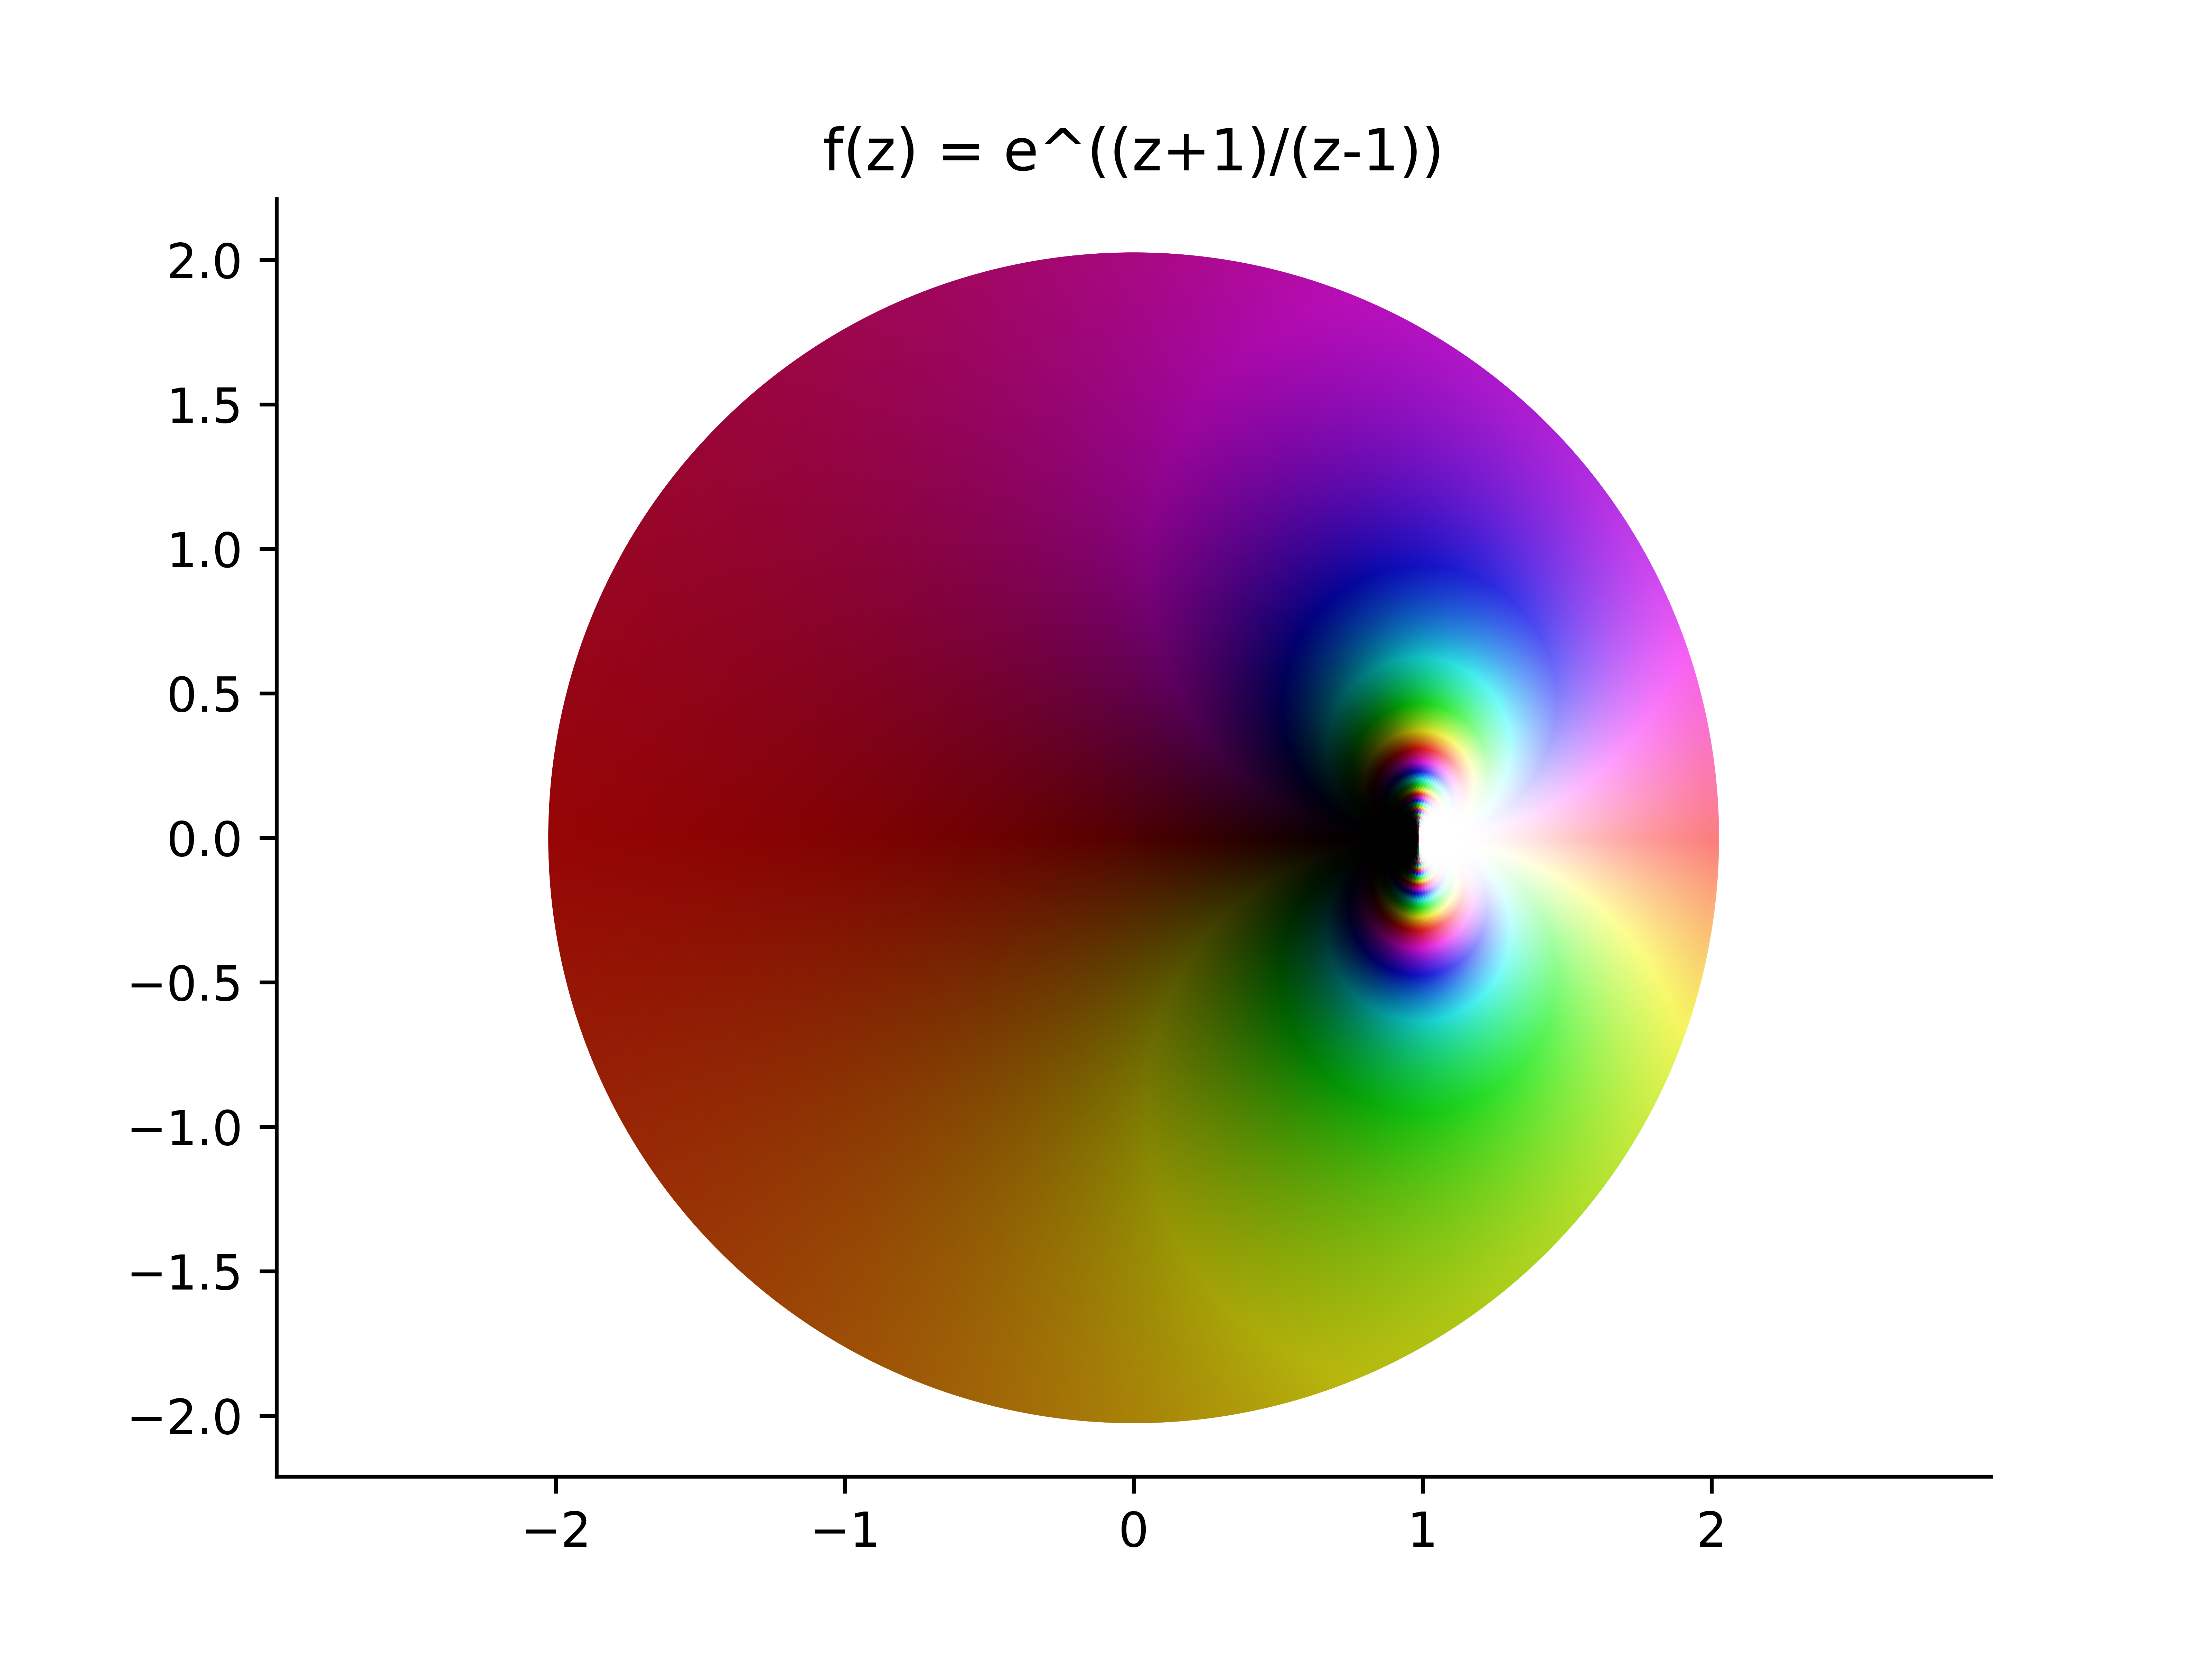
\includegraphics[width=0.7\textwidth]{../Aplicacion/e^((z+1):(z-1)).png}
        \caption{Representación de la función $\exp{\left(\frac{z + 1}{z - 1}\right)}$ en el disco unidad.}
        \label{fig:ejemplo5}
    \end{figure}

     Estudiaremos este ejemplo con más detalle en el Capítulo \ref{cap:banach}, centrándonos de nuevo en el comportamiento de la función en el punto singular $z = 1$. \\
\end{proof}

\section{Productos infinitos}

En esta sección, introducimos la noción de producto infinito convergente, relacionándola con la convergencia de una serie numérica. Esta construcción puede extenderse a productos infinitos de funciones holomorfas, lo que da lugar a nuevas familias de funciones holomorfas complejas cuando se obtienen como límite uniforme sobre compactos de productos apropiados. \\

\begin{definition}
    Sea $\{u_n\}$ una sucesión de números complejos tal que $u_n \neq 0$ para todo $n \geq n_0$. Se dice que el producto infinito $\prod_{n=1}^{\infty} u_n$ es convergente cuando el límite
    \begin{equation*}
        \lim_{N \to \infty} \prod_{n=n_0}^{N} u_n
    \end{equation*}
    existe y es distinto de cero. En este caso, se define el producto infinito como
    \begin{equation*}
        \prod_{n=1}^{\infty} u_n = \lim_{N \to \infty} \prod_{n=1}^{N} u_n. \\
    \end{equation*}
\end{definition}

\medskip

Los siguientes dos resultados nos van a permitir relacionar la convergencia de un producto infinito con la convergencia de las series, lo cual nos va a ser de gran ayuda ya que estas últimas son mucho más fáciles de manejar. \\

\begin{prop}
    Sea $\{u_n\}$ una sucesión de números complejos no nulos. Si $\lim u_n =1$ y la serie
    \begin{equation*}
        \sum_{n=1}^{\infty} \log u_n
    \end{equation*}
    converge absolutamente, es decir, $ \sum_{n=1}^{\infty} \abs{\log u_n}$ converge, entonces el producto infinito
    \begin{equation*}
        \prod_{n=1}^{\infty} u_n
    \end{equation*}
    converge absolutamente.
\end{prop}

\begin{proof}
    Si $n$ es suficientemente grande, entonces $u_n$ puede escribirse como $u_n = 1 - \alpha_n$, donde $\abs{\alpha_n} < 1$, y entonces podemos definir $\log{u_n}$ como $\log{(1 - \alpha_n)}$. Por hipótesis, se sigue que la serie
    \begin{equation*}
        \sum_{n=1}^{\infty} \log u_n = \sum_{n=1}^{\infty} \log{(1 - \alpha_n)}
    \end{equation*}
    converge. Así que las sumas parciales
    \begin{equation*}
        \sum_{n=1}^{N} \log u_n
    \end{equation*}
    tienen límite y es finito. Como la función exponencial es continua, podemos exponenciar las sumas parciales y vemos que
    \begin{equation*}
        \prod_{n=1}^{\infty} u_n = \lim_{N \to \infty} \prod_{n=1}^{N} u_n
    \end{equation*}
    existe. \\
\end{proof}

\begin{prop}
    \label{th:convergencia}
    Sea $\{\alpha_n\}$ una sucesión de números complejos tales que $\alpha_n \not = 1$ para todo $n$. Supongamos que
    \begin{equation*}
        \sum_{n=1}^{\infty} \abs{\alpha_n}
    \end{equation*}
    converge. Entonces
    \begin{equation*}
        \prod_{n=1}^{\infty} (1 - \alpha_n)
    \end{equation*}
    converge absolutamente.
\end{prop}

\begin{proof}
    Para una cantidad finita $n$, tenemos que $\abs{\alpha_n} < \frac{1}{2}$, así que $\log{(1 - \alpha_n)}$ está definido por la serie usual, y para alguna constante $C$, tenemos
    \begin{equation*}
        \abs{\log{(1 - \alpha_n)}} \leq C \abs{\alpha_n}.
    \end{equation*}
    Por tanto, el producto converge absolutamente por definición y utilizando la hipótesis de que $\sum_{n=1}^{\infty} \abs{\alpha_n}$ converge. \\
\end{proof}

Una vez que disponemos de las herramientas apropiadas para el estudio de los productos numéricos en términos de las series asociadas, se puede analizar la convergencia (absoluta y uniforme) de productos infinitos de funciones en términos de la convergencia (absoluta y uniforme) de las series correspondientes. En la siguiente sección utilizaremos este resultado para introducir los productos de Blaschke. \\

La demostración del resultado que presentamos a continuación es análoga a las de los precedentes. \\

\begin{theorem}
    Si $\{u_n\}$ es una sucesión de funciones complejas acotadas en un conjunto $A$ tales que $\sum \abs{1-u_n(z)}$ converge uniformemente en  $A$, entonces el producto $f(z) = \prod u_n(z)$ converge uniformemente en A y cumple que $f(z_0) = 0$ si y solo si existe $n_0$ tal que $u_{n_0}(z_0) = 0$.
\end{theorem}

\section{Productos de Blaschke}

Tras los ejemplos de funciones holomorfas en el disco unidad que presentamos en la primera sección, definidas mediante su serie de potencias centrada en 0 o a través de su expresión analítica explícita, utilizamos la noción de producto infinito de funciones para presentar una clase especial de funciones holomorfas y acotadas en el disco. Se trata de los productos de Blaschke, que se obtienen a través de un producto infinito de automorfismos del disco unidad. Cada uno de ellos está ligado a un valor $\alpha$ en el disco, el único punto donde el automorfismo se anula, y la convergencia del producto infinito se describe dada en términos de los distintos valores $\alpha_n$. En concreto, la sucesión $\{\alpha_n\}$ debe aproximarse rápidamente al borde del disco, como muestra el resultado que se presenta a continuación. \\

\begin{theorem}
    Sea $\{\alpha_n\}$ una sucesión en el disco unidad $\disk$ tal que $\alpha_n \not = 0$ para todo $n$ y $\sum_{n=1}^{\infty} (1 - \abs{\alpha_n})$ converge. Entonces el producto de Blaschke
    \begin{equation*}
        B(z) = \prod_{n=1}^{\infty} \frac{\alpha_n - z}{1 - \xbar{\alpha_n}z} \dfrac{\abs{\alpha_n}}{\alpha_n}
    \end{equation*}
    converge uniformemente sobre los compactos de $\disk$. La función $B(z)$ define una función holomorfa en el disco unidad que tiene los mismos ceros que $\alpha_n$. Además $\abs{B(z)} \leq 1$ y $\abs{B(e^{i \theta})} = 1$ en casi todo punto.
\end{theorem}

\begin{proof}
    Sea
    \begin{equation*}
        b_n (z) = \frac{\alpha_n - z}{1 - \xbar{\alpha_n}z} \dfrac{\abs{\alpha_n}}{\alpha_n}.
    \end{equation*}

    Por el Lema \ref{th:convergencia}, sabemos que $\prod_{n=1}^{\infty} b_n$ converge uniformemente sobre los compactos de $\disk$ a una función holomorfa que tiene los mismos ceros que $\{\alpha_n\}$ si y solo si $\sum_{n=1}^{\infty} \abs{1 - b_n}$ converge uniformemente sobre los compactos de $\disk$. Para $\abs{\alpha_n} < 1$ y $\abs{z} \leq r < 1$, se tiene

    \begin{equation*}
        \begin{split}
            \abs{1 - b_n(z)} & = \abs{1 + \dfrac{z - \alpha_n}{1 - \xbar{\alpha_n}z} \dfrac{\abs{\alpha_n}}{\alpha_n}} = \abs{\dfrac{(1 - \xbar{\alpha_n}z) \alpha_n + (z - \alpha_n) \abs{\alpha_n}}{(1 - \xbar{\alpha_n}z) \alpha_n}} = \\
                             & = \abs{ \dfrac{\alpha_n + z \abs{\alpha_n}}{\alpha_n (1 - \xbar{\alpha_n}z)}} (1 - \abs{\alpha_n}) \leq \dfrac{1 + r}{1 - r} (1 - \abs{\alpha_n}).
        \end{split}
    \end{equation*}
    pues si $\abs{\alpha_n} < 1$ y $\abs{z} \leq r$ se verifican $\abs{\alpha_n + z \abs{\alpha_n}} \leq 1+r$, y $\abs{1- \xbar{\alpha_n}z} \geq 1-\abs{\xbar{\alpha_n}}\abs{z} \geq 1-r$. \\

    Entonces para $\abs{z} \leq r < 1$, se tiene
    \begin{equation*}
        \sum_{n=1}^{\infty} \abs{1 - b_n(z)} \leq \dfrac{1 + r}{1 - r} \sum_{n=1}^{\infty} (1 - \abs{\alpha_n}),
    \end{equation*}
    y la serie $\sum_{n=1}^{\infty} \abs{1 - b_n(z)}$ converge absoluta y uniformemente en el disco cerrado de radio $r$. Por lo que $B(z) = \prod_{n=1}^{\infty} b_n$ converge uniformemente sobre los compactos de $\disk$. \\

    Como $b_n(z)$ son funciones holomorfas en $\disk$ y su producto infinito converge uniformemente en los compactos de $\disk$, se tiene que $B(z)$ define una función holomorfa en el disco unidad. Se está utilizando que la topología de la convergencia uniforme sobre compactos es la apropiada, ya que los límites en ella de elementos de $\bholomorphic{\disk}$ existen y son, de nuevo, funciones holomorfas. \\ %$f$ tiene los mismos ceros que $\alpha_n$ por la definición de producto infinito.

    Además, se cumple $\abs{B(z)} \leq 1$ por la caracterización de los automorfismos del disco unidad ya que los términos $\dfrac{\alpha_n - z}{1 - \xbar{\alpha_n}z}$ definen un automorfismo del disco unidad que lleva el disco abierto en el disco abierto y el borde en el borde. \\

    Así pues, aplicando el Teorema de Fatou, $B(z)$ tiene límites radiales $\abs{B(e^{i\theta})} \leq 1$ en casi todo punto. Para ver que $\abs{B(e^{i \theta})} = 1$ en casi todo punto, tomemos $B_n(z) = \prod_{k=1}^{n} b_k(z)$ el producto parcial. Entonces, $\frac{B}{B_n}$ es otro producto de Blaschke y
    \begin{equation*}
        \abs{\frac{B(0)}{B_n(0)}} \leq \frac{1}{2 \pi} \int_{0}^{2 \pi} \abs{\frac{B(e^{i \theta})}{B_n(e^{i \theta})}} d \theta = \frac{1}{2 \pi}  \int_{0}^{2 \pi} \abs{ B(e^{i \theta})} d \theta.
    \end{equation*}

    Tomando $n \to \infty$, obtenemos
    \begin{equation*}
         \frac{1}{2 \pi}  \int_{0}^{2 \pi} \abs{ B(e^{i \theta})} d \theta = 1,
    \end{equation*}
    y, por consiguiente, $\abs{ B(e^{i \theta})} = 1$ en casi todo punto. \\
\end{proof}

\begin{obs}
     Cada $b_n(0)$ es positivo y por lo tanto también lo es $B(0)$. \\
\end{obs}

Podemos enunciar un resultado similar al anterior si permitimos que $\alpha_n$ se anule $m$ veces, lo que significa que $B$ se anulará en los mismos puntos que $\alpha_n$. Haciendo uso de la Proposición anterior, lo que atañe a la convergencia y los límites radiales es inmediato y no precisa demostración. \\

\begin{corollary}
    Sea $\{\alpha_n\}$ una sucesión en el disco unidad $\disk$ tal que $\sum_{n=1}^{\infty} (1 - \abs{\alpha_n})$ converge. Sea $m$ el número de $\alpha_n$ iguales a cero. Entonces el producto de Blaschke
\begin{equation*}
    B(z) = z^m \prod_{\abs{\alpha_n} \not = 0} \frac{\alpha_n - z}{1 - \xbar{\alpha_n}z} \dfrac{\abs{\alpha_n}}{\alpha_n}
\end{equation*}
converge uniformemente sobre los compactos de $\disk$. La función $B(z)$ define una función holomorfa en el disco unidad que tiene los mismos ceros que $\alpha_n$. Además $\abs{B(z)} \leq 1$ y $\abs{B(e^{i \theta})} = 1$ en casi todo punto. \\
\end{corollary}

Después de la discusión anterior podemos dar una formulación general de los productos de Blaschke. \\

\begin{corollary}
    Sea $\{\alpha_n\}$ una sucesión en el disco unidad $\disk$ tal que $\sum_{n=1}^{\infty} (1 - \abs{\alpha_n})$ converge. Sea $m \geq 0$ el número de $\alpha_n$ iguales a cero, y $t \in \real$. La expresión general de un producto de Blaschke es
    \begin{equation*}
        B(z) = e^{it}z^m \prod_{\abs{\alpha_n} \not = 0} \frac{\alpha_n - z}{1 - \xbar{\alpha_n}z} \dfrac{\abs{\alpha_n}}{\alpha_n}.
    \end{equation*}
\end{corollary}
